\documentclass{ctexart}
\usepackage{graphicx}
\usepackage{amsmath}
\usepackage{amsthm}
\usepackage{amssymb}
\usepackage{fancyhdr}
\usepackage{ifthen}
\usepackage{syntonly}
\usepackage[colorlinks, CJKbookmarks=true, linkcolor=red]{hyperref}
\pagestyle{plain}
\usepackage[raggedright]{titlesec}
\newtheorem{性质}{性质}
\newtheorem{定理}{定理}
\newtheorem{推论}{推论}
\begin{document}
\title{作业}
\author{计算机科学与技术系52班 杨定澄 \and 学号:2015011274 \and E-mail:892431401@qq.com}
\date{}
\maketitle
\section*{第一题}
\subsection*{(a)}
$P(z_{i1},z_{i2},\cdots z_{in}|P(\omega_i))=P(z_{i1}|z_{i2},\cdots,z_{in},P(\omega_i))P(z_{i2}|,z_{i3},\cdots z_{in},P(\omega_i))\cdots P(z_{in}|P(\omega_i))$。由于$z_{ij}$互相独立,故$\textrm{上式}=\prod\limits_{k=1}^nP(z_{ik}|P(\omega_i))$

而事实上$P(z_{ik}=0|P(\omega_i))=1-P(\omega_i),P(z_{ik}=1|P(\omega_i)=P(\omega_i)$,综上,$P(z_{ik}|P(\omega_i)=P(\omega_i)^{z_{ik}}(1-P(\omega_i))^{1-z_{ik}}$

故$P(z_{i1},z_{i2},\cdots,z_{in}|P(\omega_i))=\prod\limits_{k=1}^nP(\omega_i)^{z_{ik}}(1-P(\omega_i))^{1-z_{ik}}$
\subsection*{(b)}
\[\frac{\partial \ln P(z_{i1},z_{i2},\cdots,z_{in}|P(\omega_i))}{\partial P(\omega_i)}=\sum_{k=1}^n \frac{z_{ik}}{P(\omega_i)}+\sum_{k=1}^n \frac{1-z_{ik}}{P(\omega_i)}\]

令$\frac{\partial \ln P(z_{i1},z_{i2},\cdots,z_{in}|P(\omega_i))}{\partial P(\omega_i)}=0$,并设$S=\sum\limits_{k=1}^n z_{ik}$,有方程$\frac{S}{P(\omega_i)}=\frac{n-S}{1-P(\omega_i)}$

解得$\hat{P}(\omega_i)=\frac{S}{n}=\frac{1}{n}\sum\limits_{k=1}^n z_{ik}$

这个结果是因为,单独针对$i$类来看,可以看做一个二项分布,也就是一个事情有$P(\omega_i)$的概率成功,$1-P(\omega_i)$的概率失败。

我们想要估算这个事情的成功率,假设实践了$n$次,有$m$次成功,一个符合我们直觉的估计是,这件事情的成功率是$\frac{m}{n}$
\section*{第二题}
假设有$n$组样本,记第$i$组样本的第$j$维向量是$x_{i,j}$,我们要确定参数$\theta=(\theta_1,\cdots,\theta_d)^T$使得$P(x_1,x_2,\cdots,x_n|\theta)$最大。
\begin{align*}
\textrm{记}L(\theta)&=\ln P(x_1,x_2,\cdots,x_n|\theta)\\
&=\ln [ \prod_{i=1}^n\prod_{j=1}^d \theta_j^{x_{i,j}}(1-\theta_j)^{1-x_{i,j}} ]\\
&=\sum_{i=1}^n\sum_{j=1}^d (x_{i,j}\ln \theta_j+(1-x_{i,j})\ln(1-x_{i,j})\\
\textrm{有}\frac{\partial L}{\partial \theta_j}&=\sum_{i=1}^n (\frac{x_{i,j}}{\theta_j}-\frac{1-x_{i,j}}{1-\theta_j})=0\\
&\Longrightarrow \sum_{i=1}^n \frac{x_{i,j}}{\theta_j}=\sum_{i=1}^n \frac{1-x_{i,j}}{1-\theta_j}\\
&\Longrightarrow \sum_{i=1}^n x_{i,j}(1-\theta_j)=\sum_{i=1}^n (1-x_{i,j})\theta_j\\
&\Longrightarrow \theta_j=\frac{1}{n}\sum_{i=1}^n x_{i,j}\\
&\Longrightarrow \hat{\theta}=\frac{1}{n}\sum_{k=1}^n x_k
\end{align*}
\section*{第三题}
\subsection*{(a)}
\begin{align*}
\textrm{记}L(p)&=\ln P(x_1,x_2,\cdots,x_d|p,\omega_1)\\
&=\ln [ \prod_{i=1}^d p^{x_i}(1-p)^{1-x_i} ]\\
&=\sum_{i=1}^d(x_i\ln p+(1-x_{i})\ln(1-p)\\
\textrm{有}\frac{dL}{dp}&=\sum_{i=1}^d (\frac{x_{i}}{p}-\frac{1-x_{i}}{1-p})=0\\
&\Longrightarrow \sum_{i=1}^d \frac{x_{i}}{p}=\sum_{i=1}^d \frac{1-x_{i}}{1-p}\\
&\Longrightarrow \sum_{i=1}^d x_{i}(1-p)=\sum_{i=1}^d (1-x_{i})p\\
&\Longrightarrow p=\frac{1}{d}\sum_{i=1}^d x_{i}\\
\end{align*}
\subsection*{(b)}
先证明该估计的无偏性:

\[E(\frac{1}{d}\sum_{i=1}^dx_i)=\frac{1}{d}\sum_{i=1}^dE(x_i)=\frac{1}{d}dp=p\]

接着要说明当$d$趋于无穷时错误概率趋于$0$,首先算该估计的方差。由于样本两两独立,故协方差均为$0$。

\[var(\frac{1}{d}\sum_{i=1}^d x_i)=\frac{1}{d^2}\sum_{i=1}^nvar(x_i)=\frac{1}{d^2}dp(1-p)=\frac{p(1-p)}{d}\]

\[\lim_{d \rightarrow \infty} var(\frac{1}{d} \sum_{i=1}^d x_i)=0\]

根据切比雪夫不等式

\[P(|p-\hat{p}| \ge \epsilon)\le \frac{var(\hat{p})}{\epsilon^2}\]

而$var(\hat{p})=0$,故错误概率为$0$。
\subsection*{(c)}
我用MATLAB分别画了$(d=11,P(T|\omega_1)),(d=111,P(T|\omega_1)),(d=11,P(T|\omega_2)),(d=111,P(T|\omega_2))$四种情况。

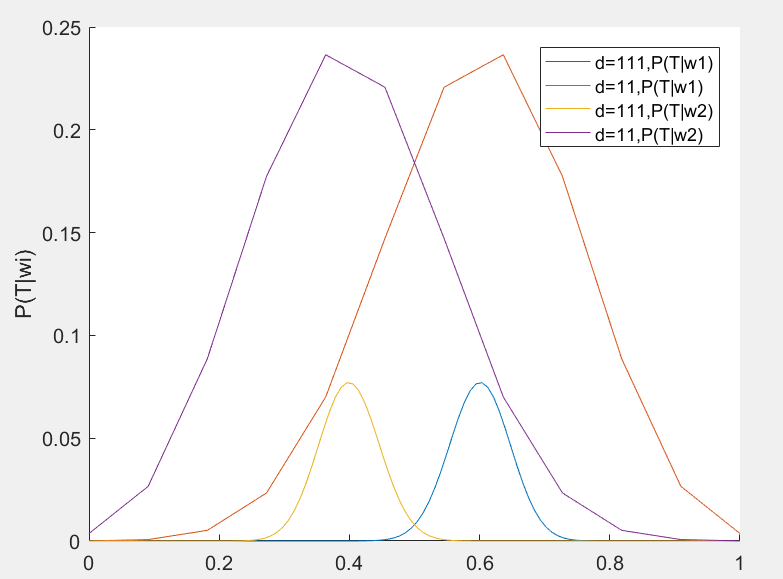
\includegraphics[width=5in]{plot.png}

也可以在plot.fig中打开或运行draw.m程序。

大概有如下几个特点:

\begin{enumerate}
\item
$d$比较小时,$P(T|\omega_i)$相对较大,这是由于此时情况比较少导致的。
\item
$d$比较小时,函数在极值点周围变化较慢;$d$比较大时,极值点可以看做是一个峰值。这验证了中心极限定理(样本不断增加,就会越来越汇聚在期望值处)
\item
$d$相同时,$P(T|\omega_1)$与$P(T|\omega_2)$会对称,这是由于概率密度函数的对称性导致的。
\end{enumerate}
\end{document}
